\documentclass{article}
\usepackage[bottom]{footmisc}
\usepackage{graphicx}
\usepackage{float}
\usepackage{titlesec}
\usepackage{amsmath}


\usepackage{makeidx}

\setcounter{secnumdepth}{4}



%\usepackage{adjustbox}  
\newcommand{\V}{\verb}
\newcommand{\x}{$\textbf{X}$}
\newcommand{\y}{$\textbf{Y}$}
\newcommand{\s}{$\textbf{S}$}
\newcommand{\A}{$\textbf{A}$}
\newcommand{\mx}{$\textbf{M}_{\textbf{X}}$}
\newcommand{\my}{$\textbf{M}_{\textbf{Y}}$}
\newcommand{\ma}{$\textbf{M}_{\textbf{A}}$}
\newcommand{\q}{$\textbf{Q}_{\textbf{1}}$}
\newcommand{\qq}{$\textbf{Q}_{\textbf{2}}$}
\newcommand{\pc}{$\textbf{PC}$}    
\newcommand{\J}{$\textbf{J}$}
\renewcommand{\thefootnote}{\roman{footnote}}


\title{FML: a VM implemented in SML}
\author{Henrik Sommerland, Oskar Ahlberg, Aleksander Lunqvist}
\date{\today}

\begin{document}
\maketitle


\begin{abstract}
For our project we have decided to build a virtual 
machine(VM) in SML.
The name FML is just an arbitrary thre letter name and has no meaning or interpertation.
The VM is a RISC machine using a Von-Neuman architecture. It has a very
minimalistic instruction set. The design of FML resembles those of older 8-bit
architectures such as the MOS 6510 and the Z80 microprocessors commonly in use
during the late 70s and early 80s. The FML machine has no ``bus width'' and 
works exclusivley with signed integers\footnote{The details of the integers
used are dependent on which SML implementation is used}. The lack of a physical
bus enables the VM to do things wich an ordinary CPU could not achive such as
reading from two registers at the same time. Even though
the cpu have very few operations (only 27) a very effective instruction set architecture
makes these operations very flexibels and there are roughly 600 valid    
instruction codes. It is also noteworthy that FML is asycrounous and has now
predefined clock frequenzy.\footnote{Allthogh for debugging purposues one can
use both manual stepping and a fixed update speed.}

So even though FML is a very minimalistic machine it is quite powerfull.
We have allso built a fully featured assembler for the FML machine.
\end{abstract}
\tableofcontents
\section{Our work}
We have tried to work as independent as possible. This has ofcourse led to some
difference in how we have commented the code, some slight differnces in naming
and indentation. The way we have chosen do describe how our programs work
differes a bit here depending on who wrote the code for the given part of the
VM.

We have not been using any form of unit testing. But instead we have done a
series of more and more complicated online tests. This due to the scale and the
complexity of the various funtions and algorithms of the project.

We have continously have meetings both with just us in the group and also some
with our assigned TA\footnote{Our TA has during this project been Tobias Neil}.
These meetings have primairly been about informing eathother about how the 
VM works and how the various components of it should be
implemented. We have then had an ongoing discussion on facebook regarding
details and problems wich we have encountered.

We have been using Git as a source code management system. We have been using
BitBucket for to host the project and troughout all of the development process
the repository has been hidden and only we in the group and our TA have had
access to the code.\\
\\
We are using an array  in the current implementation of the memory for the VM.
Now i know that it is stated in the project description that the project should
be written in a functional and pure way. I discussed with both Dave Clarke and
Tjark Weber about using a ``monad like'' structure to hide the sideffects of the
array hadling and they said that it was okay. The Signature handling the memory
is written in such a way that any other part of the program implementing the
memmory structure will not be able to se that there are any side effects. I.e
there are no semantically observable side effects of the memory structure. All
of the code would look exactly the same from ``the outside'' regardles of how we
implemented the memory.

\subsubsection{Personal notes}
In this section we will give som personal notes regarding our parts in the
project.
\paragraph{Henrik Sommerland}
I have been incharge of designing the VM and writing the assembler. I have also
written some signatures for the others in the group to help them get started. I
began work very early, as soon as we had gotten permission to start on the
project. I  began by writing the specifications for the VM.

Even though i have never had any formal education in how computer achitectures
work I have learnt a lot about it on my own. When i was younger (around 17) i
designed a 8-bit cpu from TTL logic chps (the 7400 series). It was during this
time I learned how to build a cpu. So the design of the FML machine was for me
very straight forward. I have done all of the design myself and i have not
copied anything from books or any previous designs. Allthough my way of thinking
and reasoning about cpu architectures comes primarily from my own work and the
designs of older 8-bit cpus. The design of the cpu took roughly one or two days
to finish and then there has been a continous process of ironing out bugs and
inconsitencies.

Then I started to write the assembler. From the start I had a pretty good idea
about what I wanted the assembler to do and I had a pretty good idea how to
implement it. I wrote the assembler in about three days and I then had a fully
working assembler.

After I had completed the assembler I sat out to start testing it and to write
the documentation for it. As I wrote the documentation and did more extensive
testing of the assembler I worked out the last few bugs and such in the code.

Then i started to write signature files and such for the others in the group to
get to work on. I allso started to write on the major report for the entire
program whilst guiding the others in the group.

In general I have found this project to be increadibly fun and interesting. In
the beggining I was worried that the others in the group where not going to be
able to understand how it all woked and even though it's really hard to explain
something complex wich is crystal clear in my head to other people the others in
the group have ben very enthusiastic and have really pulled trough this mammoth
of a project.


\section{The VM}
Here a informal description of the workings of the machine. For a more detailed
description se the VM specifications in the appendix.
\subsubsection{General}
The FML machine is built up as a very simple von-neuman architecture. The
machine consists ony of a few major components. It's notewhorthy that there is
no instruction decoder present. This is since all of the instruction decoding
and handling takes place within the software implementation of the machine.
The size of the memory the machine has avaliable is arbitrary and is defined at
the initilazion of the machine. Below will follow a dataflow diagram of the
machine, describing all of the components and how they can communicate.  

\begin{figure}[H]
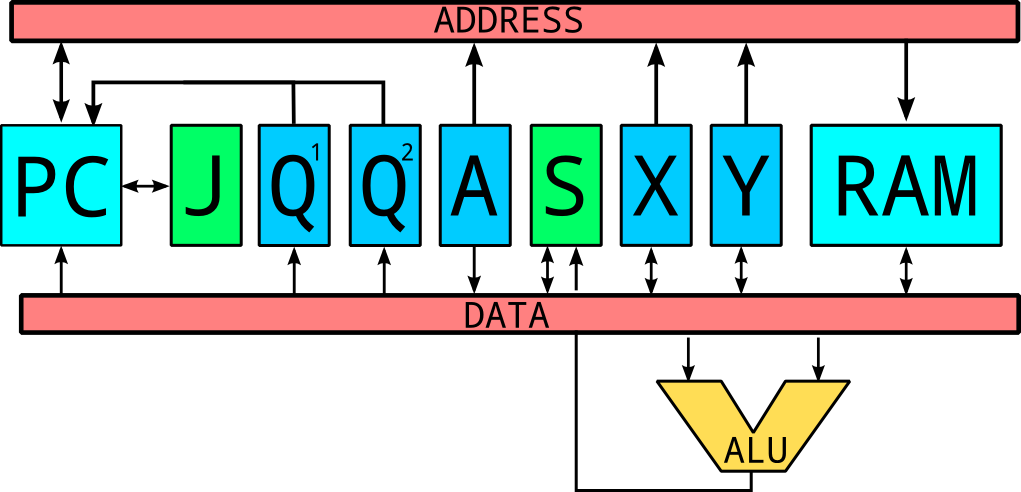
\includegraphics[width=\textwidth,height=\textheight,keepaspectratio]{Dataflow.png}
\caption{Dataflow diagram of the FML machine}
\end{figure}       

Now this image might be a little bit confusing. One should consider the two read
rectangles DATA and ADDRESS as ``viritual buses''. One can interpret the picture
as: X can both read and write from other components and be used for addressing.
Below will follow brief descriptions of the components. More indepth
descriptions are given in the appendix.

\begin{description}
  \item[X and Y] \hfill \\ 
  These are the two general purpose registers wich can be read,
  written to and used for addressing.
  \item[S] \hfill \\
  This is the general purpose stack. It can be both read and
  written to. Everytime some thing gets written to the stack it gets pushed onto the
  stack and everytime something is read from the stack the stack gets popped.
  The stack can not be used for addressing.
  \item[A] \hfill \\
  This is only a virtual register. It is read only and can be used for
  addressing. This is only used if an instructuion uses a non-register
  argument\footnote{A non-registry argument is a argument wich is not any of
  the registers, the stack, or something from the memmory. The value of A will
  (if used) be at the memmory cell directly folowing the one at wich the
  program counter is.}.
  \item[Q$^1$ and Q$^2$] \hfill \\
  These are the two interupt registers. These are very special and can only be
  written to. They will hold the adresses to wich the machine should jump if an
  prepherial component makes a interupt request. More on this later.
  \item[PC]\hfill \\
  This is the program counter. It keeps track on where in the memmory the 
  instructions are being read from. It allso handles the jumping.
  \item[J]\hfill \\
  This is the jump stack. This stack is used to store the return addresses for
  subroutine jumps. This stack can only be manipulated by the program counter.
  \item[ALU]\hfill \\
  This is not really a ALU. The machine does not have a seppareta ALU component
  but this is just here to illustrate that the all of the components which can
  be read from can be used as arguments for arithmetic and logical operations.
  All of the results from the arithmetic and logical operations are always put
  on the stack.
  \item[RAM]\hfill \\
  This is the random access memmory of the machine.
\end{description}

\subsubsection{Instruction Set Architecture}
The ISA of the VM is built in a special but simple fashion. Each instruction
corresponds to a six digit integer..
Where each digit corresponds to specific information regarding different types of opcodes. The digits counting from right
to left is: 

\begin{description}
  \item[First] Second argument
  \item[Second] First argument
  \item[Third] Arithmetic operations
  \item[Fourth] Logic operations
  \item[Fifth] Jump operations
  \item[Sixth] Special
\end{description}
This system of encoding information into each digit of the instruction makes the
implementyation of the instruction controler and the assembler much easier. It
allows for all the operation types to be grouped into numerical ranges and it
gives  a lot of flexibility. Note that some of the instructions may be invalid
and some might be nonsensical but the instruction controler crashes if a invalid
instruction is encountered. The assembler is written in such a way that it can
only generate valid instructions. So an example would be:
000401.
Where the 4 tells us that it we should perform a modulo operation, 
he 0 says that the second argument is the \x register and the last 1 says 
that the first argument is the \y register. Notice that the order of
the last two digits is reversed in respect to the order of the arguments in
the operation.
This is due to a design choise made early in the design phase. It makes the
instructions code a bit more confusing to read but it makes the assembly code
become far more intuitive.\\
For a more detailed description of the ISA se the VM specifications in the
appendix.

\section{Assembler}
\subsubsection{General}
The assembler wich we have written for the FMl machine is a very basic yet
powerfull assembler. The assembler doesnt do much more than catch invalid
opcodes and arguments. It allso enables the use of both label pointers and value
pointers. The main tasks of the assembler is the instruction code generation and
address resolution. The syntax of the assembler is inspired by the syntax for
the MOS 6510 assembly lanuage and primarily the syntax of the Turbo Assembler
for the Commodore 64. The assembler is now fully functional and there we dont
see any need to augment it or redisgning any spects of it. The assembler should
only generate valid instructions but due to a major design error in the
implementation of the VM this is not neccesarily true any more. Below a short
example of a assembly program will follow:
\begin{verbatim}
% This a simple program wich fills a part 
% of the memmory with 100 consecutive integers
% trough rellative addressing.
#start
MOV 0 x
@start_address
MOV start_addres y
#loop
MOV x $y
INC x
INC y
BLE x 100
JMP loop
HLT
\end{verbatim}
A line starting with a \V+#+ declares a label. The address of the label will
correspond to where in the code the the lebel gets declared.
A line starting with a \V+@+ declares a value. The address of the label will be
assigned independent of where in the code it apepars.
For a more indepth description of how the assembly lanuage se the Assembler part
of the description.

\subsubsection{Implementation}
\paragraph{General}
The assembler works in a fairly straight forward way. The first step in the
process of asemblying is the lexiographical analysis in wich the lines in the
text file gets tokenized. In this tage an ``intermediate structure''
\footnote{The use of the word structure here is a bit ambigous since it
actually is a structure in sml. But in this text it will reffere to an abstract
structure of data.} gets constructed.
This is an object wich contains all of the labels, values and alist of the tokenized lines. The list of 
the tokens contains tupels of
\verb+(label,offsett,token)+ wherer the lable is the last initialized label and
the offset is how many addresses away from that line the current token is. Allof
the labels and values will not be assigned an adress in this phase. It is in
theis phase where the opcodes and their arguments gets converted in to there
corresponding numerical instruction code. It is also during this phase in wich
the syntax gets checked. If a syntax error is encountered the assembler will
stop emideatly. When the lexiographical analysis has been completed a check for
duplicate pointer declaration is performed.

The next phase in the assembly is the address resolution phase. This is done in
two phases, in the first one the labels gets resolved and in the second the
values gets  resolved. It begins by first resolving the labels.
This is done by first giving the assembler a \emph{base address} wich is 
the adress of the first label. As of now the first
non comment line in the input file has to be a label since every line has to
have a label assigned to it. Then the address resolution function continues down
the intermediate sturcture and remebering wich line it is at and what its last
read label was. When it runns into a new label token it will sett the new label
to its current address and then continue on untill it has gone trough the entire
intermediate structure. After the labels have been resolved the assembler starts
to resolve the values. This is done in a very straightforward way. The assembler
just looks at the last address of the last entry in the output of the firsst
pass and looks at the last address, adds one to it and the just places the all
the values in after that address in the same order as they appeared in the file.
After all the adress has been resolved the assembler runns trough the list of
tokens and replaces every pointer token with its correct adress.

After this is completed the assembler finalizes the code by converting
everything into a list of integers wich then gets outputed to a file. And that
children is how assembly code gets turned in to machine code.

the assembler runns in linear time with respect to the number of lines in the
code. This is under the assumption that the number of lines are far greater than
the number of values and labels in the code. This is a safe assumption for any
resonably written code.

\paragraph{Flow chart}
Below a flow chart will folow for how the assembler assembler the assembles the
assembly code.
 
\begin{figure}[H]
\begin{centering}
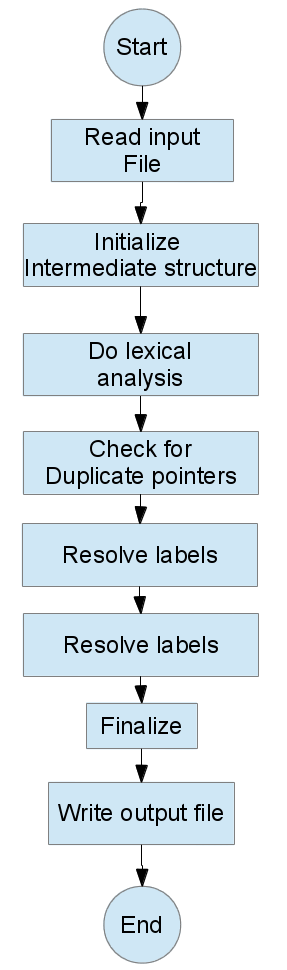
\includegraphics[width=\textwidth,height=\textheight,keepaspectratio]{assembler_flow.png}
\caption{Dataflow diagram of the assembler}
\end{centering}
\end{figure}

\newpage

\begin{figure}[H]
\begin{centering}
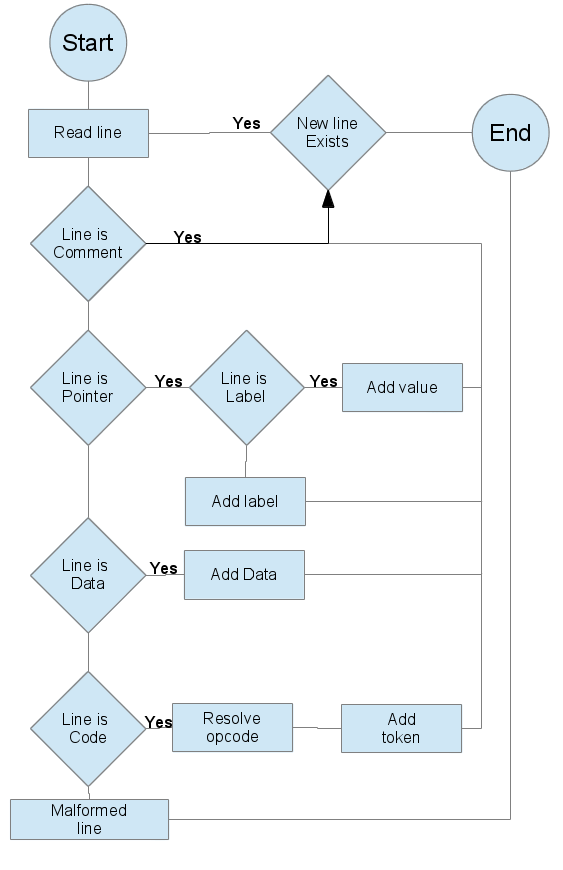
\includegraphics[width=\textwidth,height=\textheight,keepaspectratio]{lexicographical_flow.png}
\caption{Dataflow diagram of the tokenization phase}
\end{centering}
\end{figure}

\newpage

\begin{figure}[H]
\begin{centering}
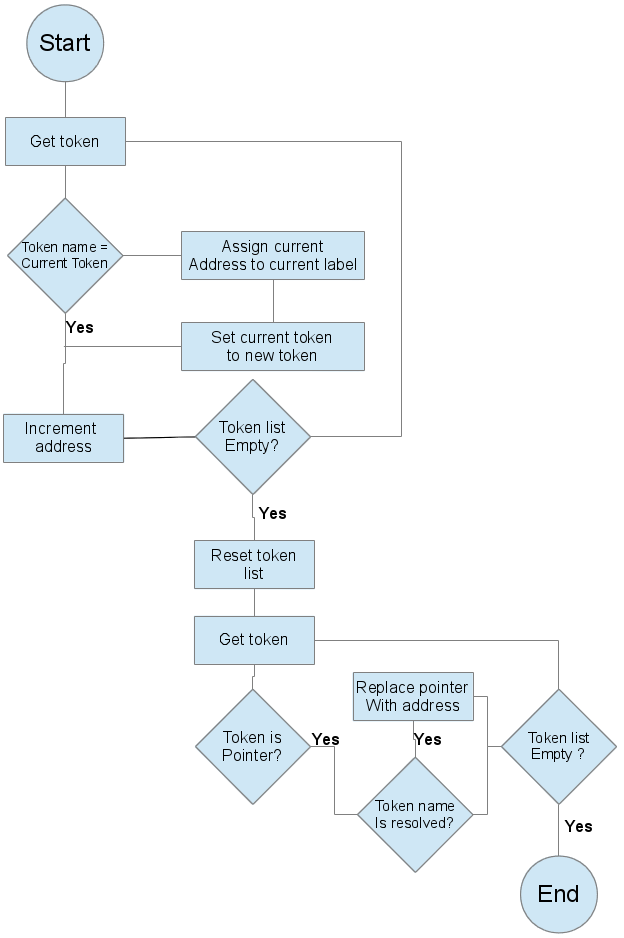
\includegraphics[width=\textwidth,height=\textheight,keepaspectratio]{address.png}
\caption{Dataflow diagram of the label address resolution}
\end{centering}
\end{figure}
\newpage
The i have not included a flowchart for the address resolution of the values or
the finalization part since these are trivial.
\paragraph{Usage}  
To use the assembler propperly one has to know how to write assembly code and
understand the detailed workings of the machine. We recomend studying both the
VM spcifications and the assembler documentation in the appendix before you
start to write programs for the machine.

The working of the assembler program is very straight forward. just frite your
assembly code in a file called \V+in.asm+ and run the \V+Assembler.sml+ file in
the sml interperter of your choosing and if there are no errors encountered during
the assembling of the program the assembeled program will be outputed to a file
named \V+out.fml+.

\section{Appendix}
\subsection{Componets.sml description}
Due to misscomunication a radicaly diffrent description of how the
Components.sml file works was written and have been included here as an
appendix.
\subsubsection{Introduction}

The following structures and signatures are present in Components.sml are the
Ram, Stack, Register and ProgramCounter.

\subsubsection{The Ram structure}
\paragraph{Synopsis} \ 
\\
signature RAM\\
structure Ram :\textgreater RAM\\

The Ram structure provides a base of the functions of a ram memory. This
structure acts as something akin to a ``monad''. It hides all of the sidefects
sued for the array handling.

\paragraph{INTERFACE} \ 
\\
    type memory = int array
	\\val initialize : int $\rightarrow$ memory 							
 	\\val getSize : (memory) $\rightarrow$ int 
    \\val write :(memory * int * int ) $\rightarrow$ memory	  				
	\\val read : (memory * int) $\rightarrow$ int							
	\\val load : (memory* int list) $\rightarrow$ memory					
	\\val writeChunk : (memory * int * (int array)) $\rightarrow$ memory
	\\val readChunk : (memory * int * int) $\rightarrow$ int array			
	\\val dump : memory $\rightarrow$ string
\paragraph{Description} \
\\
val initialize : int $\rightarrow$ memory \\	
	Initialize the ram to a memory with the size of int, when int > 0
\\
val getSize : (memory) $\rightarrow$ int\\
		Gets the size of the memory
\\
val write :(memory * int * int ) $\rightarrow$ memory\\
		write takes a memory and writes a new value of int at the pointer of the first
		int and returns the memory
\\
val read: (memory * int) $\rightarrow$ memory\\
		read takes a memory and reads the value of the place of int
\\
val load: (memory * int list) $\rightarrow$ memory\\
		load takes a list of values and loads them to the memory
\\
val writeChunk: (memory* int *( int array)) $\rightarrow$ memory \\
		writeChuck takes a memory and a start pointer and adds a chunk to the memory
\\
val readChunk: (memory * int *int) $\rightarrow$ int array \\
		readChumk takes a memory and reads a chunk form first int to the last int and gives the values as an int array
\\
val dump: memory $\rightarrow$ string\\
		dump takes a memory and returns the value as strings

\subsubsection{The Stack structure}
\paragraph{Synopsis}\
\\
signature STACK \\
structure Stack :\textgreater STACK
\\
The Stack structure provides a base for the stack part of the Pc structure.

\paragraph{INTERFACE}\
\\
	datatype stack = Stack of (int list)\\	
	val empty : stack \\
	val push : stack * int $\rightarrow$ stack\\					
	val pop : stack $\rightarrow$ stack\\						
	val top : stack $\rightarrow$ int\\						
	val isEmpty : stack $\rightarrow$ bool \\						
	val dumpStack : stack $\rightarrow$ string\\					 
	
\paragraph{Description}\
\\
	val empty : stack\\
		is a definition of a empty Stack
\\
	val push : stack * int $\rightarrow$ stack\\					
		takes a stack and adds the value of int to the stack.
\\
	val pop : stack $\rightarrow$ stack	\\					
		takes a Stack and pops the first element of the stack.
\\
	val top : stack $\rightarrow$ int\\							
		takes the stack and returns the first element of the stack
\\
	val isEmpty : stack $\rightarrow$ bool\\						
		takes a stack and checks if it is empty if it is then true else false.
\\
	val dumpStack : stack $\rightarrow$ string\\
		takes a stack, then pops the stack until its empty and returns all values as string

\subsubsection{The Register structure}
\paragraph{Synopsis} \
\\
signature REGISTER\\
structure Register :\textgreater REGISTER\\
\\
The Register structure provides a base structure of the different register that
is contained in the Pc as well the Virtual machine. The vm has two different registers.\\
\paragraph{INTERFACE} \
\\
	datatype reg = Reg of int 
\\	
	val setData : (reg * int) $\rightarrow$ reg 				
\\	val getData : reg $\rightarrow$ int						
\\	val increment : reg $\rightarrow$ reg						
\\	val decrement : reg $\rightarrow$ reg						
\\	val dumpRegister : reg $\rightarrow$ string
\paragraph{Description} \ 
\\

	val setData : (reg * int) $\rightarrow$ reg\\
		Setups a new Register \\
	val getData : reg $\rightarrow$ int	\\
		Gets the value of the reg as an int\\					
	val increment : reg $\rightarrow$ reg\\		
		Takes a reg and increment it with one.\\	
	val decrement : reg $\rightarrow$ reg\\					
		Takes a reg and decrements it with one.\\
	val dumpRegister : reg $\rightarrow$ string\\
		Takes the register and adds all elements to a string.\\

\subsubsection{The Program Counter structure}
\paragraph{Synopsis} \ 
\\
signature PROGRAM\textunderscore COUNTER\\
structure ProgramCounter :\textgreater PROGRAM\textunderscore COUNTER\\
\\
The ProgramCounter structure controls the execution flow of the VM
\\
\paragraph{INTERFACE} \ 
\\
	datatype pc = Pc of (int * Stack.stack * Register.reg * Register.reg)
\\
	val incrementPointer : (pc * int) $\rightarrow$ pc\\
	val jump : (pc * int) $\rightarrow$ pc\\
	val subroutineJump : (pc * int) $\rightarrow$ pc\\ 						
	val return : pc $\rightarrow$ pc\\	
    val interrupt : (pc * int) $\rightarrow$ pc\\
    val dumpPc : pc $\rightarrow$ string\\
\\
\paragraph{Description} \ 
\\
	val incrementPointer : (pc * int) $\rightarrow$ pc\\
		Takes a Pc and adds a int > 0\\							
	val jump : (pc * int) $\rightarrow$ pc\\
		Takes a Pc and jumps the pc counter to the value of int > 0\\
	val subroutineJump : (pc * int) $\rightarrow$ pc\\
		Takes a Pc and preforms SubrutineJump with the value of  int > 0 and adds the  value of the pointer + 1 to the stack\\						
	val return : pc $\rightarrow$ pc\\
    	Takes a pc and gets the value from the pointer and pops the stack with the value\\
	val interrupt : (pc * int) $\rightarrow$ pc\\							
		if the value of a is 1 or 2, then the value of i is added to s\\
	val dumpPc : pc $\rightarrow$ string\\
		Takes a pc and dumps the content of the pc as a string (the Pc contained a pointer, Stack, and tow registers)\\

\end{document}
